\documentclass[12pt]{article}

\usepackage{graphicx}
\usepackage[margin=1.0in]{geometry}
\usepackage{amsmath}
\usepackage{cases}
\usepackage{amsfonts}
\usepackage{amssymb}
\usepackage{grffile}
\usepackage{setspace}

\setlength\parindent{0pt}

\author{Xiaohui Chen \\EID: xc2388}
\title{M 362K Post-Class Homework 13}


\begin{document}
\maketitle
\begin{spacing}{2.0}

\section*{5-9}

$E[X]= \int_{0}^{\infty} x(1+x)^{-4} dx = \frac{1}{6}$

Therefore the answer is (A)

\section*{5-12}

From the property of probability density function, we can know that $\int_{0}^{1} cx dx = \frac{c}{2} = 1$

$\therefore c=2$

$\mu_X = E[X] = \int_{0}^{1} 2x^2 dx = \frac{2}{3}$

$E[X^2]= \int_{0}^{1} 2x^3 dx = \frac{1}{2}$

$Var[X] = E[X^2]- \left(E[X]\right)^2 = \frac{1}{2} - \frac{4}{9}= \frac{1}{18} $

$\sigma_X= \sqrt{Var[X]}= \sqrt{\frac{1}{18}} \approx 0.235702$

Let COV denotes the coefficient of variation of X

$\therefore COV= \frac{\sigma_X}{\mu_X} \approx 0.353553$

\section*{5-14}

\subsection*{(a)}

$E[X]= \int_{1}^{8} \frac{x}{7} dx = 4.5$

$E[X^2] = \int_{1}^{8} \frac{x^2}{7} dx = \frac{73}{3}$

$\sigma_X= \sqrt{Var[X]} = \sqrt{E[X^2]- \left( E[X] \right)^2 } \approx 2.02073$

\subsection*{(b)}

$E[\sqrt{X+1}] = \int_{1}^{8} \frac{\sqrt{X+1}}{7} = \frac{18}{7}-\frac{4 \sqrt{2}}{21} \approx 2.30205$

\section*{5-21}

\begin{figure}

\centering
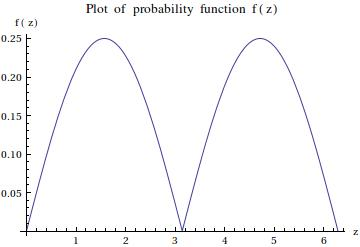
\includegraphics[width=4in]{out1}

\caption{Plot of f(z)}
\label{out1}

\end{figure}

The plot of the probability density function is shown in Figure \ref{out1}

$\therefore E[Z] = \int_{0}^{2\pi} z\frac{|\sin z|}{4} dx = \pi $

From Figure \ref{out1}, we know that when $ 0 \le z \le pi $, $F_X(x)= -\frac{\cos z}{4} + \frac{1}{4} $

When $\pi \le z \le 2\pi $, $F_X(x)= \frac{1}{2} - \frac{\cos (z- \pi)}{4} + \frac{1}{4}= \frac{3}{4} + \frac{\cos (z-\pi)}{4}$

This means

\begin{numcases}{F_X(x)}
-\frac{\cos z}{4} + \frac{1}{4} & if $0 \le z \le \pi$\\
\frac{3}{4} + \frac{\cos (z-\pi)}{4} & if $\pi \le z \le 2\pi$
\end{numcases}

When $z=\pi$, $F_X(x)=0.5$

$\therefore z_{0.5} = \pi$

From Figure \ref{out1}, the modes are $\frac{\pi}{2}$ and $\frac{3\pi}{2}$

\section*{5-25}

We know that 

\begin{numcases}{f(x)}
0 & if $x<0$ or $x>3$\\
\frac{1}{9} \left(4 x-x^2\right) & if $0 \le x \le 3$
\end{numcases}

Therefore $f'(x)=\frac{1}{9} (4-2 x) $

To get $f'(x)=0$, $x=2$

$f(2)=\frac{4}{9}>0$

Therefore $x_{mode}= 2$

The answer is (D)

\end{spacing}
\end{document}
